
\chapter{Model of Solution System\label{chpt:models}}

Computing models of solvents are broadly divided into two types: those
treating the solvent as a continuous medium (implicit models) and
those describing the individual solvent molecules (explicit models).
In the implicit model, the solvent is characterized only by the dielectric
constant $\varepsilon$ and contains an artificial-shaped cavity.
The explicit models can have more specific scales. Within the scope
of classical mechanics, the most expensive method can be the explicit model %Uncertain if these are the names of two explicit models
which includes flexible and polarizable, while in computational chemistry, less precise
models often have wider usage (for example, the proteins are treated
in the unity of residues). As the theory of liquids was firstly established
for spherical atom-like solvent particles, the model adopted by the
theory is a rigid molecule, only depending on its position and orientation,
i. e. there is no relative movement within the solvent particles.
This approximation has been proven reasonable \citep{Gray-Gubbins}.
In this section, we will give a brief introduction of the implicit model in order
to facilitate later discussion on solvation free
energy corrections. We will then focus on the rigid solvent model. The
flexible and polarizable models will also be briefly mentioned in
order to understand the limits of the rigid model. 


\section{Continuum Solvation Models}

Continuum models, which are popular in QM calculations, consider the
solvent as a uniform polarizable medium with dielectric constant $\varepsilon$,
with the solute $M$ placed in the cavity within this medium \citep{Jensen}
(figure \ref{fig:Reaction-field-model}) 

\begin{figure}[h]
\begin{centering}
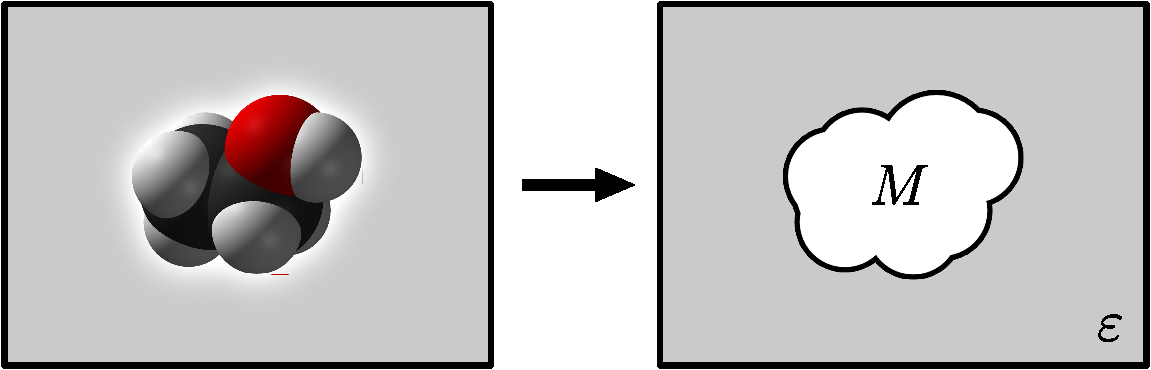
\includegraphics[width=0.75\columnwidth]{_figure/reaction-field-model_2}
\par\end{centering}

\caption{Continuum model\label{fig:Reaction-field-model}}
\end{figure}


The solvation Gibbs free energy according to this model is:
\begin{equation}
\Delta G_{\mathrm{solvation}}=\Delta G_{\mathrm{cavity}}+\Delta G_{\mathrm{dispersion}}+\Delta G_{\mathrm{elec}}\label{eq:cm}
\end{equation}
where $\Delta G_{\mathrm{cavity}}>0$ is the energy needed to create
a hole in the medium, and $\Delta G_{\mathrm{dispersion}}$ is the
dispersion interaction, which is roughly the van der Waals energy
$\Delta G_{\mathrm{vdW}}<0$ between the solvent and solute. In principle,
there may also be a repulsive component, and the dispersion term is sometimes
denoted as dispersion / repulsion. $\Delta G_{\mathrm{elec}}<0$ is the
contribution of electrostatic interaction, introduced by electric
charge distribution of $M$ which polarizes the medium, and the action
back of the medium on the molecule (reaction field). 

The initial two terms in eq. (\ref{eq:cm}) are linked to the configuration
of the first solvation shell. It is reasonable to consider this proportional
to the number of solvent molecules in the first solvation shell.

The magnitude of the free energy effect associated with any first solvation shell
phenomenon can, in an initial approximation, be considered proportional
to the number of solvent molecules in the first solvation shell. \citep{Cramer_1999_implicit_model}.
The key to a continuum treatment of these effects is to recognize
that this number, after averaging over solvent configurations, is
a non-integer continuous function of solute geometry that is characteristic
for a given solute in a given solvent at a given temperature. Furthermore,
it can be calculated as the area of a hyper-surface that passes through
the middle of the region occupied by the first shell of the solvent when
treated as a continuous medium. This is the essence of the concept of solvent-accessible surface
area (SASA) \citep{SAS_1,SAS_2} which is calculated as the area
traced out by the center of a ball rolling over the surface of a solute,
where the radius of the ball is the effective half-width of the first
solvent shell (\textasciitilde{}1-2 A for water). 

The van der Waals surface area is the surface of the union of the
spherical atomic surfaces defined by the van der Waals radius of each
component atom in the molecule. The solvent accessible surface area
 is the surface area of a biomolecule that is accessible to
a solvent. SASA is typically calculated using a sphere (of solvent)
of a particular radius to 'probe' the surface of the molecule. 

The reaction field models can differ in the size and shape of the cavity,
the definition of dielectric constant $\varepsilon$, the description
of solute $M$ (classical or ab initio), as well as the way to calculate
the free energy contributions. The definition of cavity varies from
the simplest sphere or ellipsoid to interlocking spheres located on
each nucleus which together define a van der Waals surface. The energy
required to create the cavity and the stabilization due to van der
Waals interactions between the solute and solvent together is usually
assumed to be proportional to the surface area of the cavity

\begin{equation}
\Delta G_{\mathrm{cavity}}+\Delta G_{\mathrm{dispersion}}=\gamma S_{\mathrm{cavity}}+\beta
\end{equation}
or parameterized by having a constant $\xi$ specific for each atom
type, with the $\xi$ parameters being determined by fitting to experimental
solvation data:
\begin{equation}
\Delta G_{\mathrm{cavity}}+\Delta G_{\mathrm{dispersion}}=\sum_{i}^{\mathrm{atoms}}\xi_{i}S_{i}
\end{equation}


The dielectric constant $\varepsilon$ is the only parameter characterizing
the solvent. It is normally a constant value, but for some purposes it can
depend on the distance from the solute $M$. The models and methods
to calculate the electrostatic contribution $\Delta G_{\mathrm{elec}}$
have varied greatly according to its usage. Here we list the most common
examples.


\subsection{Poisson–Boltzmann methods}

The Poisson-Boltzmann equation

A second order differential equation that gives an exact description
of the %Part of this sentence seems to be missing

This equation cannot be solved analytically for complex geometries
(such as electrostatic interactions in a dielectric medium. cav
pol vdw protein)

Therefore, it is done numerically using numerical methods, such as
finite differences.

The Poisson-Boltzmann equation is a second-order differential equation describing
the connection between the electrostatic potential $\Phi$, the charge
distribution $\rho$ and the dielectric constant $\varepsilon$.

\begin{equation}
\nabla\cdot(\varepsilon(\mathbf{r})\nabla\phi(\mathbf{r}))=-4\pi\rho(\mathbf{r})
\end{equation}


Note that the dielectric “constant” may depend on the position. When
it is independent of the position (i.e. truly a constant), eq. (14.52)
becomes eq. (14.53).

\begin{equation}
\nabla^{2}\phi(\mathbf{r})=-\frac{4\pi}{\varepsilon}\rho(\mathbf{r})
\end{equation}


If the charge distribution is a point charge, the solution of eq.
(14.53) reduces to the Coulomb interaction. 

The Poisson equation can be modified by taking into account a (thermal)
Boltzmann distribution of ions in the solvent. The negative ions will
accumulate where the potential is positive (and vice versa) subject
to a thermal fluctuation. The charge densities from a collection of
ions with charges q and -q and concentration c are given by eq. (14.54).

\begin{equation}
\begin{array}{c}
\rho_{+}=qce^{-q\phi/kT}\\
\rho_{-}=-qce^{-q\phi/kT}
\end{array}
\end{equation}


The addition of these contributions to eq. (14.52) leads to the Poisson–Boltzmann
Equation (PBE).

\begin{equation}
\begin{array}{r}
\nabla\cdot(\varepsilon(\mathbf{r})\nabla\phi(\mathbf{r}))-\kappa^{2}\left(\dfrac{kT}{q}\right)\sinh\left(\dfrac{q\phi(\mathbf{r})}{kT}\right)=-4\pi\rho(\mathbf{r})\\
\kappa^{2}=\dfrac{8\pi q^{2}I}{kT}
\end{array}
\end{equation}


Here $I$ is the ion strength of the solution, and the $\kappa^{2}$
factor is inversely related to the Debye-Hueckel length, measuring
how far the electrostatic effects extend into the solution. The $sinh(q\phi(\mathbf{r})/kT)$
term only applies for the region corresponding to the solvent, i.e.
for \textbf{$\mathbf{r}$} outside the cavity. Since $q\phi(\mathbf{r})/kT$
is dimensionless, the PBE is often written in terms of a reduced potential
$u$ instead.

\[
\nabla\cdot(\varepsilon(\mathbf{r})\nabla\phi(\mathbf{r}))-\kappa^{2}\sinh\left(u(\mathbf{r})\right)=-4\pi\rho(\mathbf{r})
\]


All of these equations ((14.52)–(14.57)) are differential equations
that must be solved numerically, typically by a grid representation,
and the results give information about the electrostatic potential
at any point in space, which is also used by later theories. It can
be mapped onto the surface of the solute where it may suggest regions
for interaction with other polar molecules. It can also be used for
generating the reaction field, defined as the difference between the
potential in the presence of a solvent (e = 78) and in vacuum (e =
1), i.e. freac = fsolv - fvac. Multiplication of the reaction field
with the solute charges in either a continuous ($\rho$) or partial
charge ($Q$) description gives the electrostatic component of the
free energy.

\begin{equation}
\Delta G_{\mathrm{elec}}=\frac{1}{2}\int\mathrm{d}\mathbf{r}\rho(\mathbf{r})\phi_{\mathrm{reac}}(\mathbf{r})
\end{equation}


\begin{equation}
\Delta G_{\mathrm{elec}}=\frac{1}{2}\sum_{i}Q(\mathbf{r}_{i})\phi_{\mathrm{reac}}(\mathbf{r}_{i})
\end{equation}



\subsection{Born/Onsager/Kirkwood models }

For certain special cases, however, the Poisson equation (14.52) can
be solved analytically, and this forms the basis for many approximate
models for estimating the electronic component in eq. (14.49).

The simplest reaction field model is a spherical cavity, where only
the lowest order electric moment of the molecule is taken into account.
For a net charge $q$ in a cavity of radius $a$, the difference in
energy between a vacuum and a medium with a dielectric constant of
$\varepsilon$ is given by the Born model.

\begin{equation}
\Delta G_{\mathrm{elec}}(q)=-\left(1-\frac{1}{\varepsilon}\right)\frac{q^{2}}{2a}
\end{equation}


It can be noted that the Born model predicts equal solvation energies
for positive and negative ions of the same size, which is not the
observed behavior in solvents such as water. Furthermore, the reciprocal
dependence on the dielectric constant means that the calculated solvent
effect is sensitive to the variation of e in the low dielectric limit
but virtually unaffected by large differences in the high dielectric
limit. Changing e from 1 to 2 gives a factor of 1/2 in eq. (14.59)
but there is virtually no difference between a solvent with a dielectric
constant of 30 (e.g. acetonitrile) and one with a dielectric constant
of 78 (e.g. water), although in actual experiments there may be a
significant difference.

The interaction between point charges is given by the Coulomb potential,
with e being a dielectric constant.

\begin{equation}
E_{\mathrm{el}}(R^{AB})=\frac{Q^{A}Q^{B}}{\varepsilon R^{AB}}
\end{equation}


Using partial atomic charges in eq. (14.59) is often called the generalized
Born model, which has been used especially in connection with force
field methods in the Generalized Born/Surface Area (GB/SA) model.
In this case, the Coulomb interaction between the partial charges
(eq. (2.20)) is combined with the Born formula by means of a function
$f_{ij}$ depending on the internuclear distance and Born radii for
each of the two atoms, $a_{i}$ and $a_{j}$.

\begin{equation}
\Delta G_{\mathrm{elec}}(Q_{i},Q_{j})=-\left(1-\frac{1}{\varepsilon}\right)\frac{Q_{i}Q_{j}}{f_{ij}}
\end{equation}


\begin{equation}
f_{ij}=\sqrt{r_{ij}^{2}-a_{ij}^{2}e^{-D}}
\end{equation}


$a_{ij}^{2}=a_{i}a_{j}$, $D=\frac{r_{ij}^{2}}{4a_{ij}^{2}}$

The effective Born radius for a given atom depends on the nature and
position of all the atoms.

The dipole in a spherical cavity is known as the Onsager model, which
for a dipole moment of m leads to an energy stabilization given by
eq. (14.61). (14.61) The Kirkwood model 68 refers to a general multipole
expansion in a spherical cavity, while the Kirkwood–Westheimer model
arises for an ellipsoidal cavity.

The Born/Onsager/Kirkwood models are widely used, for example in Marcus
theory for electron-transfer reactions, solvatochromism, electronic
structure in solution, and bio-molecules, i.e., proteins as well as nucleic
acids in water. \citep{hirata_molecular_2004}

Generalized Born. A pair-wise approximation to the PB theory

The Born formula generalized to a system of many atoms of arbitrary
shape is called the generalized Born model. The generalized Born equation
captures the physics of the Poisson-Boltzmann equation, while improving
the speed of calculations. • For atoms in a molecule, they also interact
with the solvent, but part of the solvent has now been replaced by
the other atoms of the molecule. The basic idea is to assign to each
atom an effective radius such that the solvation free energy can
be calculated using the Born formula. • So, the most important consideration
when using any GB-method is to accurately calculate effective Born
radii.

Accurate calculations of the Born radii can be obtained from the
Poisson-Boltzmann equation, since

Poisson-Boltzmann solvers (accurate but numerical and slow). • Generalized
Born models (faster, can be analytical). 

The idea of a distributed multipole expansion to represent the charge
distribution is also employed by the so-called generalized Born (GB)
approach to continuum solvation. In this instance, however, only monopoles
(i.e., atomic partial charges) are employed and instead of solving
the Poisson equation with this charge distribution, one uses the generalized
Born approximation, 41,44,88,96,211,214-226 which when used with
the dielectric descreening algorithm of {[}Still et al. 1990{]} has
been demonstrated to give results very close to those obtained from
solution of the Poisson equation 227-232 or from explicit molecular
simulations.233 

Density functional methods based on the minimization of polarization
density have been introduced as well. \citep{Marchi_2001}


\subsection{Other models adopted widely in QM calculation}

The critical physical concept for treating solute polarization in
solution is the reaction field. The reaction field is the electric
field exerted on the solute by the solvent that has polarized.

The critical physical concept for treating solute polarization in
solution is the reaction field. This is the electric
field exerted on the solute by the solvent that it has polarized. Including
this in the solute, Hamiltonian predicts a new (“distorted”) solute
electronic structure, which further alters the polarization of the
solvent. Iterating to self-consistency is called the self-consistent
reaction field (SCRF) method. \citep{Cramer_1999_implicit_model}

PCM. An alternative to the use of finite differences or finite elements
to discretize the differential operator is to use boundary element
methods. The most popular of these is the polarized continuum model
(PCM), developed primarily by the Pisa group of Tomasi and co-workers,3,142-145
which casts the quantum mechanical SCRF equations into a boundary
element problem with apparent surface charges (ASCs) on the solute
cavity surface. There are currently three different approaches for
carrying out PCM calculations: the original method, called dielectric
PCM142,143 (D-PCM); an alternative model in which the surrounding
medium is modeled as a conductor instead of a dielectric146 (C-PCM,
cf. the COSMO model below); and an implementation whereby the PCM
equations are recast in an integral equation formalism147,148 (IEF-PCM).
The latter method has lent itself to the calculation of various molecular
gradient and response properties, as detailed in section 4.2.

The SCRF models \citep{Jensen,scrf}
are widely used by theoretical chemistry applications, owing to the
popularity of the Gaussian toolkit. 

The Polarizable Continuum Model (PCM) using the integral equation
formalism variant (IEFPCM) 

Other available models are IPCM, which uses a static isodensity surface
for the cavity, the Self-Consistent Isodensity PCM (SCIPCM) model {[}Foresman96{]},
and the Onsager model {[}Kirkwood34, Onsager36, Wong91, Wong91a, Wong92,
Wong92a{]}, which places the solute in a spherical cavity within the
solvent reaction field.

The term SCRF is quite generic and it does not by itself indicate
a specific model.

PCM

CPCM Performs a PCM calculation using the CPCM polarizable conductor
calculation model {[}Barone98, Cossi03{]}.

Dipole Performs an Onsager model reaction field calculation.

IPCM Performs an IPCM model reaction field calculation. Isodensity
is a synonym for IPCM.

SCIPCM Performs an SCIPCM model reaction field calculation, i.e. the
SCRF calculation uses a cavity determined self-consistently from an
isodensity surface.


\section{Model potential of rigid molecule}

First let us define what we mean by classical fluids. These are fluids
for which the thermal de Broglie wavelength...

Here we present the model frequently used in the theory of liquids \citep{Hensen-McDonald,Gray-Gubbins}.

This case is important only for little solvent of atom size, where
quantum effect cannot be ignored.

As there's no chemical interaction of solvent

For water, most of the publications have already shown... at the approximation
level in this thesis, we have good reason to ignore quantum effect.

It should be noted that quantum effect appears at low temperatures
and for atom-size molecules. Here we don't discuss...

$u(\mathbf{r},\mathbf{\Omega_{1}},\mathbf{\Omega_{2}})$ pair potential
of solvent model, depends on intermolecular separation and orientations.
The polyatomic solvent model used in this thesis is based on 3 approximations:

Rigid molecule assumption, Classical treatment of translational and
rotational motions, and pair

However, for important solvents such as H20 and NH3, the rotational
potential energy effects become non-negligible at room temperature.
P11

quantum corrections 

for MD and IEM, we also use these approximation, 

It is quite realistic for small solvent molecules, such as ... as
their vibrational states are too huge compared to kT and ...

This assumption implies that the solvent molecule stays in its ground
vibrational state, which is quite realistic for some small solvents
that have large separation of vibrational states compared to $k_{\mathrm{B}}T$.
For water, the ratio of $T/\theta_{\mathrm{v}}$ at 298K, where $\theta_{\mathrm{v}}=h\nu/k$
is the characteristic vibrational temperature, is 2290K \citep{Gray-Gubbins}. 

rotational temperature 40.1K

That diverges the huge amount of rigid water models {[}ref{]}, and
the non-rigidity {[}ref{]} and quantum effect {[}ref{]} are also well
studied.

vibrational motions energy to great \marginpar{margin}

ignore quantum effets

This assumption fits for many small molecule solvents, such as H2O,
N2, CO, CO2, etc. In these cases, the characteristic vibrational temperature
$\theta_{\mathrm{v}}$ is quite large compared to the temperature
$T$; that is to say, the molecules will stay in their ground vibrational
state \citep{Gray-Gubbins}. Also the internal rotational ... is too
small can be averaged


\subsection{Interaction of spherical particles}

The simplest model of a fluid is the hard sphere model, with the pair
potential
\begin{equation}
u(r)=\begin{cases}
\infty & r<d\\
0 & r>d
\end{cases}
\end{equation}
where $d$ is the hard-sphere diameter. \textcolor{red}{This model
can represent some physical systems, such as ... }However, the absence
of attractive force \textcolor{red}{...} .

More realistic neutral particle models, like Lenard-Jones model, have
a potential energy curve that has the same shape as the real interaction
of rare gases, as shown in figure .

\begin{figure}[h]
\begin{centering}
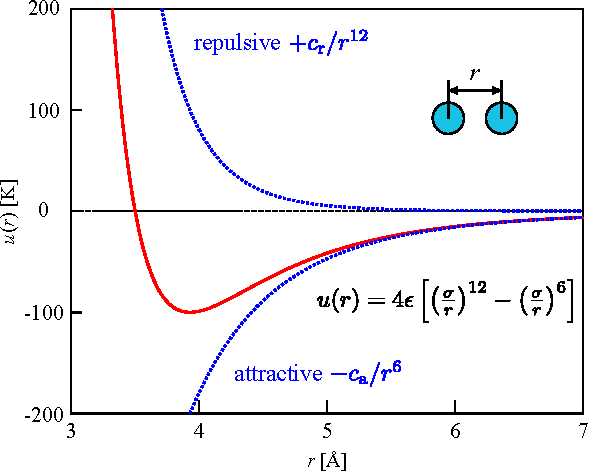
\includegraphics[scale=0.82]{_figure/lj-centre}
\par\end{centering}

\caption [LJ pair potential]{A Plot of Potential Energy versus Internuclear
Distance for the Interaction between Two Gaseous Hydrogen Atoms.} At
large distances, both attractive and repulsive interactions are small.
As the distance between the atoms decreases, the attractive electron–proton
interactions dominate, and the energy of the system decreases. At
the observed bond distance, the repulsive electron–electron and proton–proton
interactions just balance the attractive interactions, preventing
a further decrease in the internuclear distance. At very short internuclear
distances, the repulsive interactions dominate, making the system
less stable than the isolated atoms.\label{fig:LJ-pair-potential}}
\end{figure}


Lennard-Jones (LJ) interaction

\begin{equation}
u_{LJ}(r)=4\varepsilon\left[\left(\frac{\sigma}{r}\right)^{12}-\left(\frac{\sigma}{r}\right)^{6}\right]
\end{equation}
$r$ is the distance from central to central. All terms in the multipole
series represent attractive contributions to the potential. The leading
term, varying as $r^{-6}$, describes the dipole-dipole interaction.
Higher-order terms represent dipole-quadrupole ($r^{-8}$), quadrupole-quadrupole
($r^{-10}$) interactions, and so on, but these are negligible compared
to $r^{-6}$. The short-range interaction is difficult to calculate
, and is defined as $r^{12}$ in LJ model. The collision diameter
$\sigma$ (of unity {[}$\textrm{\AA}${]}) is the separation of particles
where $u(r)=0$, and $\epsilon$ is the well depth of the potential
(of unity $\mathrm{kJ/mol}$), where the minimum occurs at $r_{\min}=2^{1/6}\sigma$
and $u(r_{\min})=-\epsilon$ ,\textcolor{red}{{} ...}. These two parameters
can be measured by experimentation. 

Electrostatic interaction between charged particles coulomb

Three-body interaction

Polar liquids where dipole-dipole interaction is superposed on the
spherically symmetric potential
\begin{equation}
u(1,2)=u_{0}(r)-\boldsymbol{\mu}_{1}\cdot\mathbf{T}(\mathbf{r})\cdot\boldsymbol{\mu}_{2}
\end{equation}
where $\mathbf{r}$ is the vector separation of the molecular centers,
$u_{0}(r)$ is the spherically symmetric term as discussed above,
$\boldsymbol{\mu}_{i}$ is the dipole moment vector of particle $i$
and $\mathbf{T}(\mathbf{r})$ is the dipole-dipole interaction tensor:
\begin{equation}
T(\mathbf{r})=3\mathbf{r}\mathbf{r}/r^{5}-\mathbf{I}/r^{3}
\end{equation}
where $\mathbf{I}$ is the unit tensor.

Models in which the molecule is represented by a set of discrete interaction
sites. The total potential energy is a sum of spherical interaction
potentials. Let $\mathbf{r}_{i\alpha}$ the coordinates of site $\alpha$
in molecule $i$. the total intermolecular potential energy is
\begin{equation}
u(1,2)=\frac{1}{2}\sum_{\alpha}\sum_{\beta}u_{\alpha\beta}(\left|\mathbf{r}_{2\beta}-\mathbf{r}_{1\alpha}\right|)
\end{equation}


The full treatment of molecular fluid is shown below.


\subsection{Rigid molecule model}

The rigid molecular approximation assumes that the intermolecular
potential $\mathcal{U}(\mathbf{r}^{N},\mathbf{\Omega}^{N})$ depends
only on the positions of the $N$ molecular centers $\mathbf{r}^{N}\equiv\mathbf{r}_{1}\mathbf{r}_{2}\ldots\mathbf{r}_{N}$
and on their orientation $\mathbf{\Omega}^{N}$, where $\mathbf{\Omega}\equiv(\Theta,\Phi,\Psi)$
represents the Euler angles (figure \ref{fig:Euler angles}).

\begin{figure}[h]
\begin{centering}
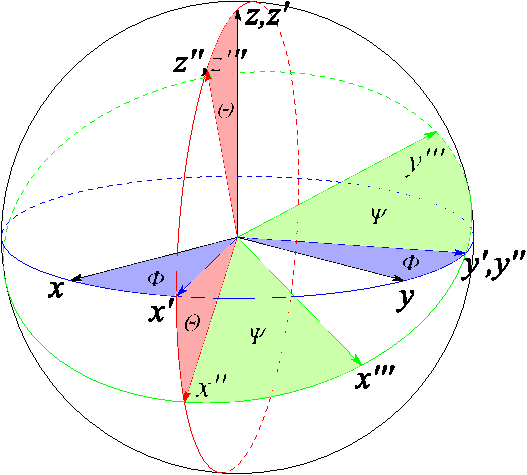
\includegraphics[scale=0.7]{_figure/euler_sphere}
\par\end{centering}

\caption [Euler angles]{The result basis vectors of the new orientation are
obtained by 3 sequential operations: (1) A rotation $\phi$ $(0<\phi<2\pi)$
about the $z$-axis, bringing the frame of axes from the initial position
S into the position ... (2) A rotation $\theta$ $(0<\theta<\pi)$
about the $y$-axis of the frame S' (3) A rotation $\psi$ $(0<\psi<2\pi)$
about the $z$-axis of the frame...\label{fig:Euler-angles}}
\end{figure}


The choice of center is often the LJ center ... ?

Pairwise additivity of intermolecular forces

The multi-body potential is often not easily dismissed, and can be taken into
account by an effective pair potential.

The effective pair potential can be measured by experiments \citep{Gray-Gubbins}
or being semi-empirical with statistical mechanical calculations.

We assume 

According to the rigid particle approximation, the pair potential
\[
\mathcal{U}(\mathbf{r}^{N},\mathbf{\Omega}^{N})=\frac{1}{2}\sum_{i\neq j}u(\mathbf{r}_{ij},\mathbf{\Omega_{i}},\mathbf{\Omega_{j}})=\sum_{i<j}u(\mathbf{r}_{ij},\mathbf{\Omega_{i}},\mathbf{\Omega_{j}})
\]


only depends on the intermolecular separation $\mathbf{r}$ and on
the molecular orientations $\mathbf{\Omega}_{1}$ and $\mathbf{\Omega}_{2}$,
\marginpar{According to the rotational invariance, $u$ can also be reduced to
$u(r,\boldsymbol{\omega_{1}},\boldsymbol{\omega_{2}})$, when $\mathbf{r}$
is referred to as polar axis.} The dependence on orientations gives properties such as...P5

This equation is quasi-exact for low density gases. The three and more
body term decreases rapidly, but it is not exact for dense fluids.

higher order corrections

\[
\mathcal{U}(\mathbf{r}^{N},\mathbf{\Omega}^{N})=\sum_{i<j}u(ij)+\sum_{i<j<k}u(ijk)+\sum_{i<j<k<l}u(ijkl)+...
\]


Three-body omission can cause surface tension problems. 
Other forces such as magnetic, multipolar, dispersion and induction
intermolecular forces are usually negligible compared to the $u_{\mu\mu}$. 

Coulomb point charge interaction

\begin{equation}
u(\mathbf{r},\mathbf{\Omega_{1}},\mathbf{\Omega_{2}})=\sum_{\alpha\beta}\frac{q_{\alpha}q_{\beta}}{r_{\alpha\beta}}
\end{equation}


Lots of models are calculated with LJ and coulomb interaction. 

site-site model

Three-body interactions


\subsection{SPC/E water and other water models}

As water is ...

There are 

The sites can placed elsewhere other than the center of atom. The more site numbers,
the more precise it becomes.

\begin{figure}[h]
\begin{centering}
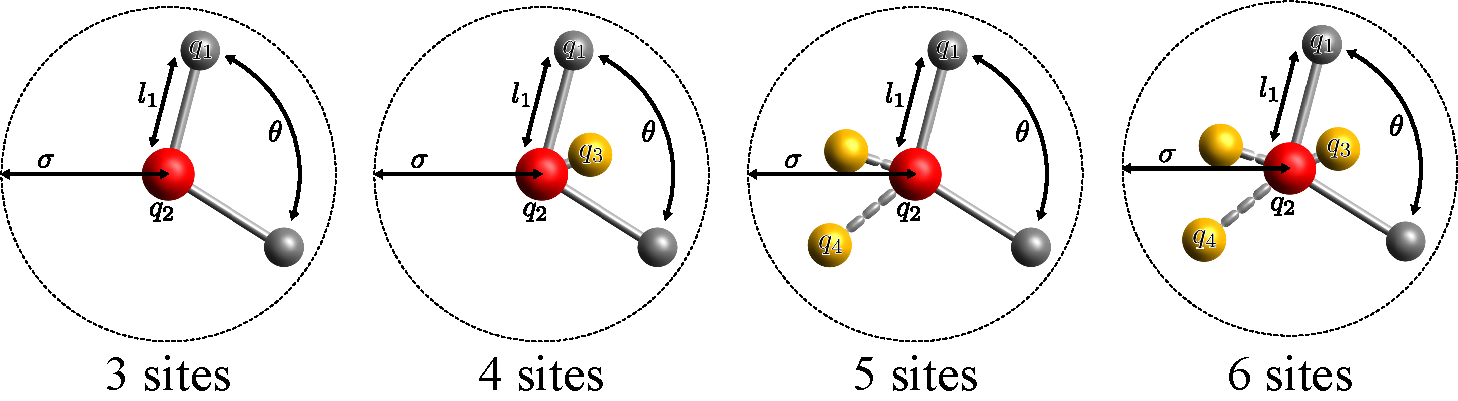
\includegraphics[width=0.75\columnwidth]{_figure/water}
\par\end{centering}

\caption{Water models\label{fig:Water-models}}
\end{figure}


Model all atom

numerical density, dielectric constant vary with temperature

In this thesis, we use the extended simple point charge model (SPC/E)
of water \citep{SPC/E} as a solvent. It is a 3-site water model. The
electrostatic interaction is modeled using Coulomb's Law and the dispersion
and repulsion forces using the Lennard-Jones potential. Any similar
model possessing \textcolor{red}{...} is compatible with this theory,
as acetonitrile is used in {[}ref{]}.

The SPC/E model adds an average polarization correction to the potential
energy function:

\[
E_{\mathrm{pol}}=\frac{1}{2}\sum_{i}\dfrac{(\mu-\mu^{0})^{2}}{\alpha_{i}}
\]
where $\mu$ is the dipole of the effectively polarized water molecule
(2.35 D for the SPC/E model), $\mu^{0}$ is the dipole moment of an
isolated water molecule (1.85 D from experiment), and $\alpha_{i}$
is an isotropic polarizability constant, with a value of 1.608 \texttimes{}
10-40 F m2. Since the charges in the model are constant, this correction
just results in adding 1.25 kcal/mol (5.22 kJ/mol) to the total energy.
The SPC/E model results in a better density and diffusion constant
than the SPC model.

The SPC/E model is successful in ... 

The parameters are listed in table \ref{tab:SPC/E}, compared with
its relative SPC model.

DC \citep{Kusalik_1994_dc_spc/e}

\begin{table}
\begin{tabular}{|c|c|c|c|c|c|c|c|c|c|c|}
\hline 
 &  &  &  &  &  &  &  &  &  & \tabularnewline
\hline 
\hline 
SPC &  &  &  &  &  &  &  &  &  & \tabularnewline
\hline 
SPC/E &  &  &  &  &  &  &  &  &  & \tabularnewline
\hline 
experiment &  &  &  &  &  &  &  &  &  & \tabularnewline
\hline 
\end{tabular}

\caption{Parameters for SPC and SPC/E water\label{tab:SPC/E}}
\end{table}



\subsection{Model flexible and polarizable}

Extra degrees of freedom

interaction site can deal with non-rigidity of water

polarization

the full force field in classical

Many atoms--> expensive Long runs required to equilibrate solvent
to solute Often solvent and solute are not polarizable. Large fluctuations
due to use of small system size 


\section{Model of solute}

The model of solute also gives an influence to the energy and structure
of solvation. The compromise to have a better model of solvent or
solute is debatable, as it varies according to the application. For
example, we never use a quantum solvent model in the case of an implicit
solute since this would not be profitable even if the solute is of simple geometry
(wall). In the case of molecular solutes, we generally require the
solute to have a model at the same  or more precise scale of description
(figure \ref{fig:Hierarchy-of-models}).

\begin{flushright}
\begin{figure}[h]
\raggedleft{}%
\begin{minipage}[t]{1.1\columnwidth}%
\begin{center}
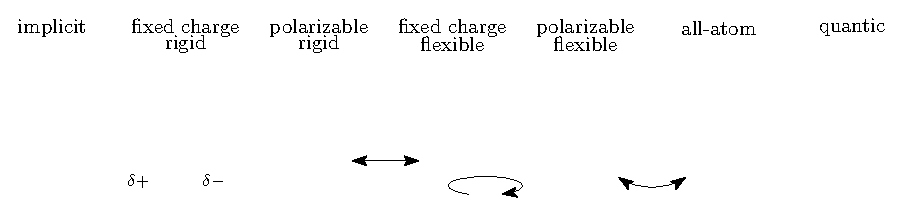
\includegraphics[width=1\columnwidth]{_figure/solute}
\par\end{center}%
\end{minipage}\caption{Hierarchy of models\label{fig:Hierarchy-of-models}}
\end{figure}

\par\end{flushright}

Most of \acs{QM} calculations in apolar solvents (toluene, etc.)
use implicit SCRF model, or even without solvent correction, and
this has proven to work well. The interaction between solute and
solvent is mainly the electrostatic interaction as described above.
Therefore 

The quantum interaction 

In this thesis, we use also rigid model to describe solute to be coherent
with IET, which cannot treat the solvent and solute in different scale
of description. 

Polarizable, flexible model, and coupling with QM is described in
perspective.
